\subsection{Purpose}
\label{intro:purpose}
This document specifies the Software Requirements Specification for the TaskList for Tomboy Project.
It describes scope of the system, both functional and non-functional requirements for the software, system interfaces and existing previous solutions.


\subsection{Scope}
\label{intro:scope}
The project TaskList is an Addin for Tomboy that will enhance Tomboy with the possibility to do task management. The user should be able to create and manage tasks with possible further more complex subtasks as well as lists of tasks.
There should be the possibility to enhance simple tasks entries with optional arguments such as due dates and priority.
The user should be able to use Tomboy intuitively as a task management system for daily usage, without prior explanation or documentation. The Addin should integrate nicely within the existing concepts and GUI elements of Tomboy.

This is how the final result could look like. Figure \ref{gui} is only a draft, trying to visualize how the integration into Tomboy can be accomplished. You can see a checkbox before each task to mark this particular task as done, along with the corresponding priorities on the left side and due dates on the right side.
\begin{figure}[h]
  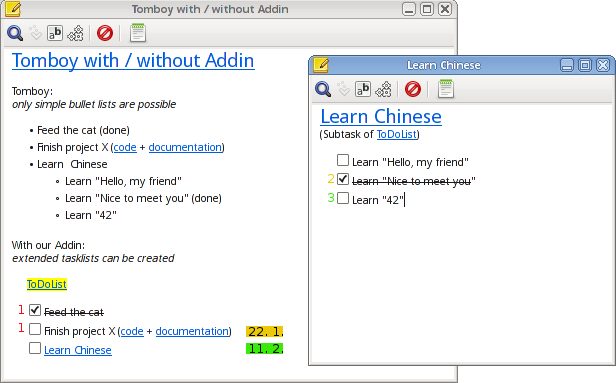
\includegraphics[width=\textwidth]{graphics/Screenshot_cropped_edited.png}
  \caption{GUI mockup}
  \label{gui}
\end{figure}


\subsection{Definitions, acronyms and abbreviations}
\label{intro:definitions}

\begin{objects}
	% Make sure to maintain alphabetical order
	\object{CLI}{Common Language Infrastructure}
	\object{C\#}{C-Sharp}
	\object{GTK}{GIMP ToolKit}
	\object{GTK\#}{Gtk Sharp}
	\object{GUI}{Graphical User Interface}
\end{objects}


\subsection{Glossary}
\label{intro:glossary}

\begin{objects}
	% Make sure to maintain alphabetical order TODO => order these ;-)
	\object{Addin}{An extension for a particular Product that can be enabled and disabled, as needed.}
	\object{Cross Platform}{Attribute conferred to computer software which is implemented and inter-operates on multiple computer platforms.}
	\object{C-Sharp}{Programming Language for the CLI Standard.}
	\object{GIMP ToolKit}{A cross platform widget library for creating GUIs.}
	\object{GNOME}{A desktop environment (a graphical user interface that runs on top of a computer operating system) composed entirely of free and open source software.}
	\object{GTK Sharp}{GTK Language Bindings for C\#}
	\object{Mono}{Cross Platform .NET Compatible Open Source implementation of the CLI Standard.}
	\object{Task}{A single activity that can be checked off when finished. Can possibly include Subtasks.}
	\object{Subtask}{A Task that has to be finished in order for another Task to be able to complete.}
	\object{Task List}{A collection of Tasks that may or may not be related.}
	\object{Tomboy}{A free and open-source desktop notetaking application written for Unix-like (including Mac OS X) and Microsoft Windows systems. Tomboy is part of GNOME and written in C\# using Gtk\#.}
	\object{User}{Any Person who uses Tomboy.}
	\object{.NET Framework}{Microsofts Implementation of the CLI Standard.}
\end{objects}


\subsection{References}
\label{intro:references}
%TODO insert link to requirements PDF, and possibly E-Mail conversations with Max / Sandy

\subsection{Overview}
\label{intro:overview} %TODO crosscheck and specify the text below
Chapter 2 defines the general product functions, intended application, constraints to be respected and
the assumption made in order to define requirements.

Chapter 3 specifies functional (Section 3.1) and non-functional requirements (all other sections),
usability, reliability, security, performance and maintainability considerations and requirements to a
level of detail sufficient to enable designers to design a system to satisfy these requirements and
testers to test that the system satisfies these requirements.

Chapter 4 contains index, appendices and supporting information.

The document is structured according to the IEEE 830-1998 standard [IEEE-830].
